\documentclass[11pt]{scrartcl}

\usepackage[sexy]{evan}
\usepackage{import}
\usepackage[table]{xcolor}
\usepackage{xfp}

\newcommand{\gad}{\textcolor{yellow}{$\bigstar$}}
\newcommand{\bad}{\textcolor{red}{$\bigstar$}}

\definecolor{dcol0}{HTML}{C8E6C9}
\definecolor{dcol1}{HTML}{D4E9B3}
\definecolor{dcol2}{HTML}{E5ED9A}
\definecolor{dcol3}{HTML}{FFF59D}
\definecolor{dcol4}{HTML}{FFE082}
\definecolor{dcol5}{HTML}{FFCC80}
\definecolor{dcol6}{HTML}{FFAB91}
\definecolor{dcol7}{HTML}{F49890}
\definecolor{dcol8}{HTML}{E57373}
\definecolor{dcol9}{HTML}{D32F2F}

\makeatletter
\newcommand{\getcolorname}[1]{dcol#1}
\makeatother

\newcommand{\dif}[1]{%
    \edef\colorindex{\number\fpeval{floor(#1)}}%
    \edef\fulltext{#1}%
    \colorbox{\getcolorname{\colorindex}}{%
        \ifnum\colorindex>8
            \textbf{\textcolor{white}{\,\fulltext\,}}%
        \else
            \textbf{\textcolor{black}{\,\fulltext\,}}%
        \fi
    }%
}
% Variable para dificultad (inicial 0)
\newcommand{\thmdifficulty}{0}

% Comando para asignar dificultad antes del problema
\newcommand{\problemdiff}[1]{\renewcommand{\thmdifficulty}{#1}}

% Estilo del problema que incluye dificultad antes del título
\declaretheoremstyle[
    headfont=\color{blue!40!black}\normalfont\bfseries,
    headformat={%
      \dif{\thmdifficulty}\quad \NAME~\NUMBER\ifx\relax\EMPTY\relax\else\ \NOTE\fi
    },
    postheadspace=1em,
    spaceabove=8pt,
    spacebelow=8pt,
    bodyfont=\normalfont
]{problemstyle}

    \declaretheorem[style=problemstyle,name=Problema,sibling=theorem]{problema}
    \declaretheorem[style=problemstyle,name=Problema,numbered=no]{problema*}

\definecolor{yellow4}{RGB}{255, 206, 0}

\title {Puntos Notables: Angle Chasing}

\author{Emmanuel Buenrostro}


\begin{document}
\maketitle

En este entrenamiento vamos a ver distintas configuraci\'ones conocidas, pero centrandonos en propiedades que salen principalmente con \'angulos (incluido ver lados iguales con isosceles/tangentes, ciclicos, paralelogramos, etc).
 
Nota: Cualquier cosa de esas puedes checarla en este \href{https://sopaconk.github.io/PONTEAENTRENAR/Mis_propias_listas/OMMJAL-FEM/Angle%20Chasing/Angle_Chasing.pdf}{pdf}
\section{Centros del triangulo}
En un triangulo $ABC$ algunos centros del triangulo son:
\begin{itemize}

    \item \textit{\textbf{H}, ortocentro}: Es la intersecci\'on de las tres alturas.

    \item \textit{\textbf{O}, circuncentro}: Es la intersecci\'on de las tres mediatrices, es el centro de la circunferencia que contiene a los puntos $A,B,C$

    \item \textit{\textbf{I}, incentro}: Es la intersecci\'on de las tres bisectrices interiores, es el centro de la circunferencia que es tangente interiormente a los tres lados del triangulo.
    
    \item \textit{\textbf{$I_A$}, $A$-excentro}: Es la intersecci\'on de la bisectriz interior de $A$, y las bisectrices exteriores de $B$ y $C$, es el centro de la circunferencia tangente interiormente a los lados $AB,AC$ y exteriormente al lado $BC$. (Analogo para \textit{\textbf{$I_B, I_C$}})

\end{itemize}



\section{$H$}

\subsection{Existe $H$}
Primero vamos a probar que $H$ existe, es decir:
\begin{exercise} [$H$ existe]
Demuestra que las tres alturas de un triangulo concurren.
\end{exercise}


\begin{claim}
Sea $H'$ la intersecci\'on de las alturas de $B$ y $C$, entonces $AH'$ es la altura desde $A$.
\end{claim}

\begin{proof}
Sean $B',C'$ los pies de altura desde $B,C$, respectivamente. Por los \'angulos de 90 que se forman podemos notar los siguientes ciclicos: 
\[ BC'B'C \text{ y } AC'HB' \]

\begin{center}
    
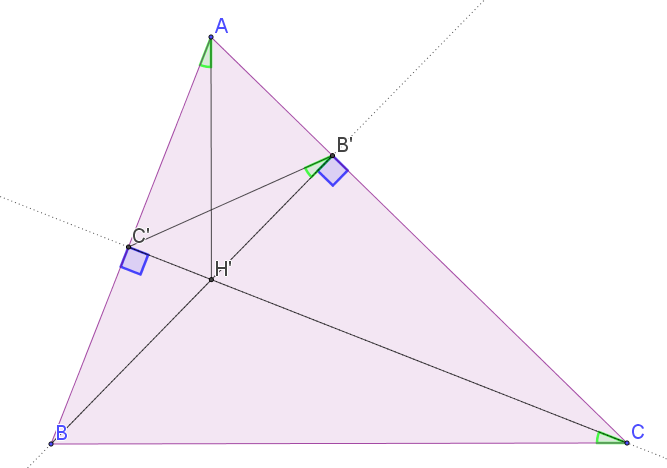
\includegraphics[scale=0.8]{PNAC1.png}
\end{center}

Entonces queremos probar que $AH' \perp BC$, entonces queremos probar que:
\[\angle BAH' = 90-\angle ABC = 90-\angle C'BC=\angle C'CB\]

Pero por los ciclicos sabemos que:
\[\angle BAH'= \angle C'AH'=\angle C'B'H= \angle C'B'B =\angle C'CB\]

Demostrando lo que queriamos probar y que $H'=H$.

\end{proof}

Entonces, en la prueba demostramos los siguientes ciclicos \footnote{Los que no vienen explicitamente en la prueba son analogos}

\[AC'HB', C'HA'B, A'CB'H \text{ y } AB'A'B, BC'B'C, CA'C'A \]

\begin{center}
    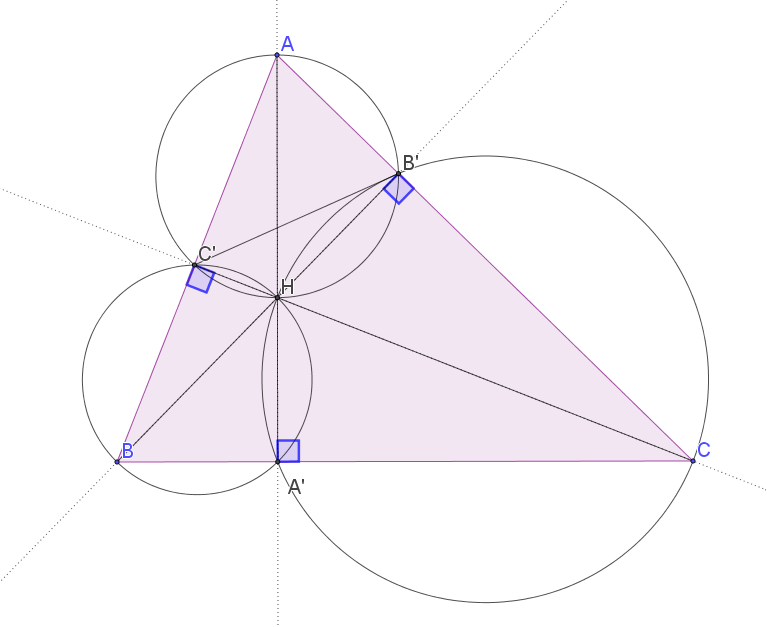
\includegraphics[scale=0.4]{PNAC2.png}
    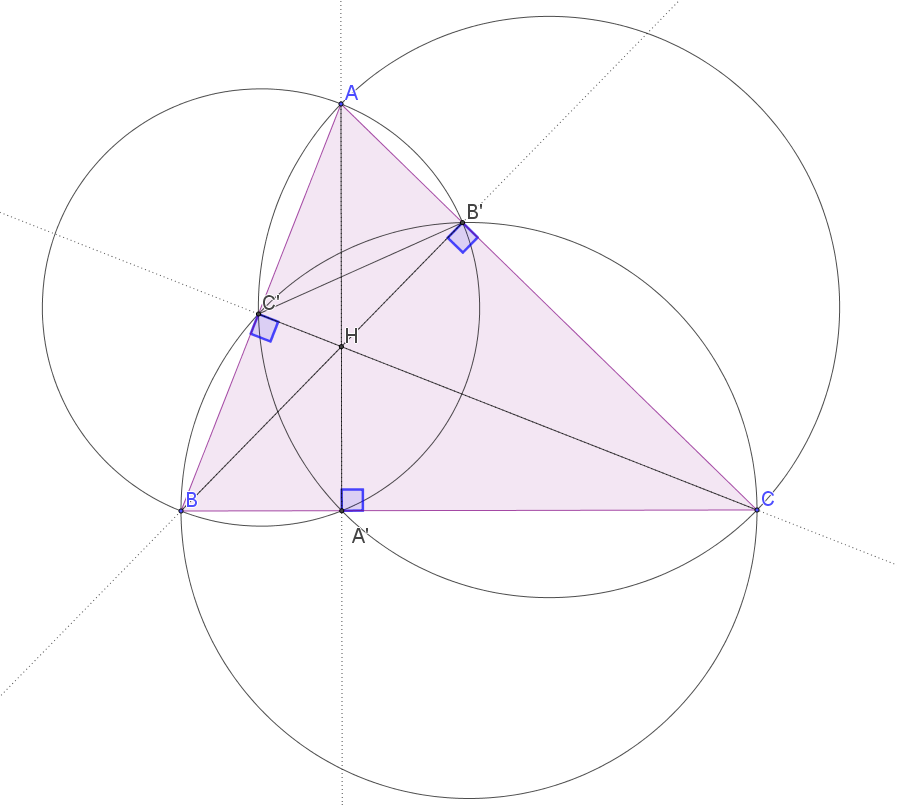
\includegraphics[scale=0.4]{PNAC3.png}
\end{center}

\subsection{Division de Angulos}

Los ciclicos antes mencionados nos dan las siguientes igualdades de \'angulos:

\begin{align*}
\angle ABH = \angle ACH &= \alpha \\
\angle BAH = \angle BCH &= \beta \\
\angle CAH = \angle CBH &= \gamma
\end{align*}

Donde nombrar cada uno de estos \'angulos nos sirve para poder hacer cuentas con los \'angulos
y esto es muy util e importante al momento de resolver problemas. \\

Algo que cumplen es $\alpha+\beta+\gamma=90\dg$

\begin{center}
    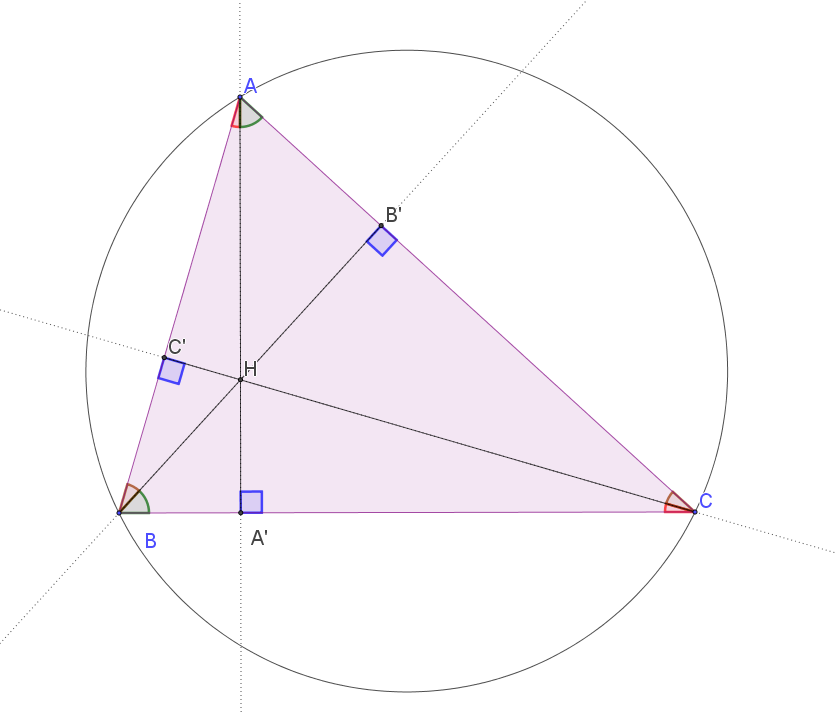
\includegraphics[scale=0.6]{PNAC11.png}
\end{center}




\subsection{Mas propiedades}

Los siguientes son propiedades de la configuraci\'on que vale la pena ver:

\begin{itemize}
    \item Sea $Y$ la reflexi\'on de $H$ sobre $BC$, demuestra que $Y$ esta en el circulo de $ABC$.
    \item Sea $M$ el punto medio de $BC$ y sea $X$ la reflexi\'on de $H$ sobre $M$. Demuestra que $X$ esta en el circulo de $ABC$.
    \item $XY \parallel BC$.
    \item $BHCX$ es un paralelogramo
    \item $AX$ es diametro de el circuncirculo de $ABC$.
    \item Sea $Q$ la intersecci\'on de $HM$ con $(ABC)$, demuestra que $QAB'HC'$ es ciclico.
\end{itemize}

\begin{center}
        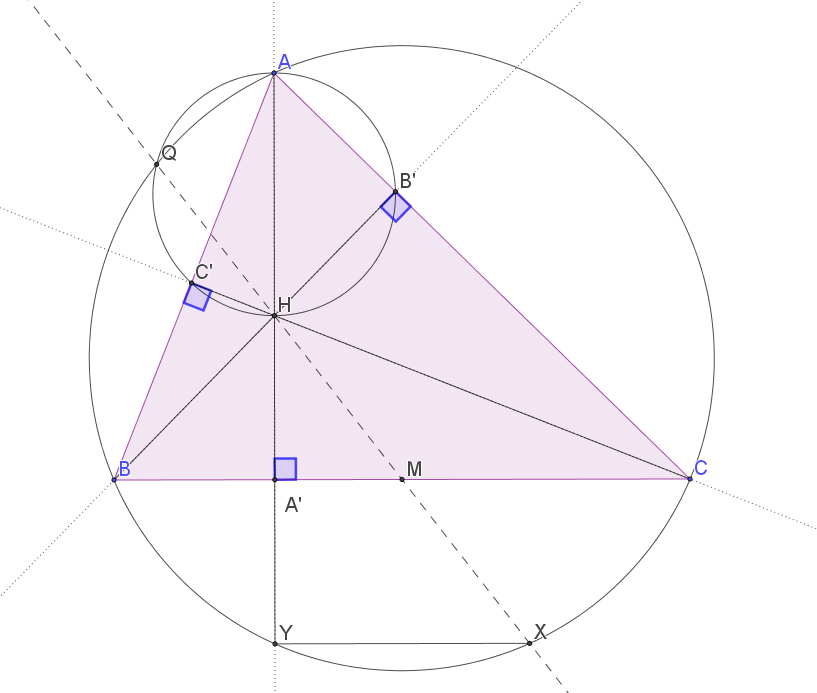
\includegraphics[scale=0.8]{PNAC9.png}
    \end{center}


\section{$O$}

\subsection{Mediatrices}

En las propiedades de $H$ usabamos el circuncirculo de $ABC$, pero ¿como sabemos que realmente existe?, vamos a demostrarlo.

Primero vamos a definir las mediatrices. 
\begin{definition}
    La mediatriz de $PQ$ es el lugar geometrico de todos los puntos $X$ tales que $XP=XQ$.
\end{definition}

Okey, esta definici\'on suena algo no tan bonito, pero vamos a ver que en realidad es lo mismo que esto:
\begin{claim}
    La mediatriz de $PQ$ es la recta perpendicular a $PQ$ que pasa por el punto medio de $PQ$. 
\end{claim}

\begin{remark*}
    Viendo la parte de \'angulos en esto, los puntos $X$ en la mediatriz cumplen que $\angle XPQ=\angle XQP$.
\end{remark*}

\begin{proof}
    Para demostrar esto tenemos que ver dos direcciones.
    \begin{itemize}
        \item Todos los puntos $X$ que cumplen $XP=XQ$ estan en la recta perpendicular a $PQ$ que pasa por el punto medio de $PQ$.
        \item Todos los puntos que estan en la recta perpendicular a $PQ$ que pasa por el punto medio de $PQ$, cumplen que $XP=XQ$.
    \end{itemize}

    \begin{center}
        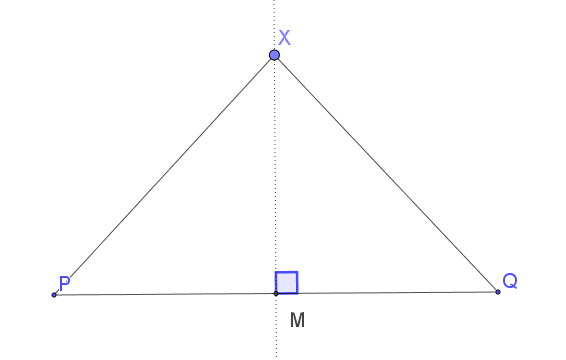
\includegraphics[scale=0.7]{PNAC4.png}
    \end{center}

    Para la primer parte, si $XP=XQ$, entonces sea $M'$ el pie de altura de $X$ hacia $PQ$.
    Como $XP=XQ$ y $\angle XM'P=\angle XM'Q=90\dg$ entoces los triangulos $XM'Q, XM'P$ son congruentes y $M'P=M'Q$, y el unico punto en la recta $PQ$ que cumple
    que $M'P=M'Q$ es el punto medio de $PQ$, probando que todos los puntos $X$ estan en la recta perpendicular a $PQ$ que pasa por el punto medio de $PQ$. \\


    Para la segunda parte, si $X$ esta en la recta perpendicular a $PQ$ que pasa por el punto medio de $PQ$, entonces si $M$ es el punto medio de $PQ$ 
    y como $MP=MQ$, $\angle XMP=\angle XMQ= 90\dg$ se tiene que $XMP, XMQ$ son congruentes y $XP=XQ$ probando la segunda parte. 

\end{proof}

\subsection{Existe $O$}

Entonces ahora para probar que $O$ existe tenemos que ver que las tres mediatrices concurren.

\begin{claim}
    En un triangulo $ABC$ las mediatrices de $AB,BC,CA$ concurren.
\end{claim}

\begin{proof}
    Sea $O'$ la intersecci\'on de la mediatriz de $AB$ y $AC$, entonces queremos probar que $O'$ esta en la mediatriz de $BC$.

      \begin{center}
        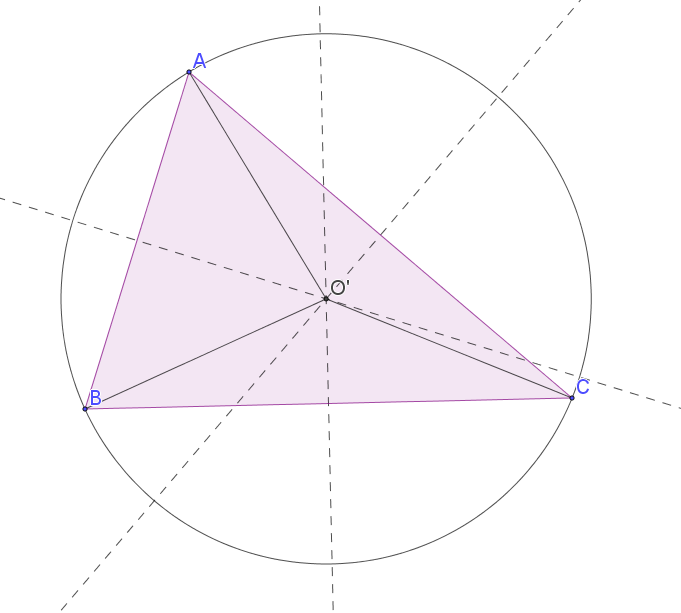
\includegraphics[scale=0.6]{PNAC5.png}
    \end{center}

    Como $O'$ esta en la mediatriz de $AB,AC$ entonces 
    \[O'B=O'A \text{ y } O'A=O'C\]
    Entonces $O'B=O'C$ y $O'$ esta en la mediatriz de $BC$. \\

    Entonces $O'=O$.
\end{proof}

Adem\'as con esto probamos que existe un punto $O$ tal que $OA=OB=OC=R$, entonces tomando un circulo centrado en $O$ y radio $R$ tenemos 
un circulo que pasa por $A,B,C$, el circuncirculo. \\


\subsection{Divisi\'on de \'Angulos}

Al igual que con $H$ podemos nombrar \'angulos iguales, que esta vez se obtienen de los isosceles con $OA=OB=OC$.

\begin{align*}
    \angle CBO = \angle BCO &= \alpha \\
    \angle ACO= \angle CAO &= \beta \\
    \angle BAO = \angle ABO &= \gamma
\end{align*}

Algo que cumplen es $\alpha+\beta+\gamma=90\dg$

\begin{center}
        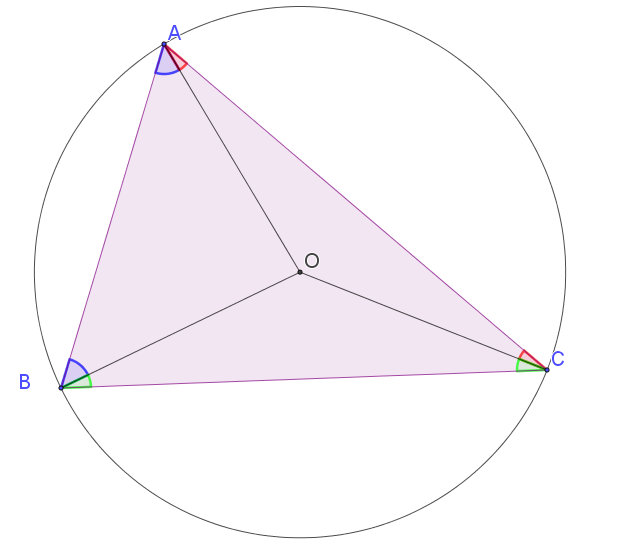
\includegraphics[scale=0.6]{PNAC12.png}
    \end{center}

\subsection{M\'as propiedades}

Algunas propiedades importantes de $O$ junto con $H$ son:

\begin{itemize}
    \item Sea $M$ el punto medio de $BC$, sea $X$ la reflexion de $H$ sobre $M$, entonces $A,O,X$ son colineales.
    \item $\angle BAH=\angle CAO$ \footnote{Esto se le dice $AH, AO$ son isogonales}
\end{itemize}

    \begin{center}
        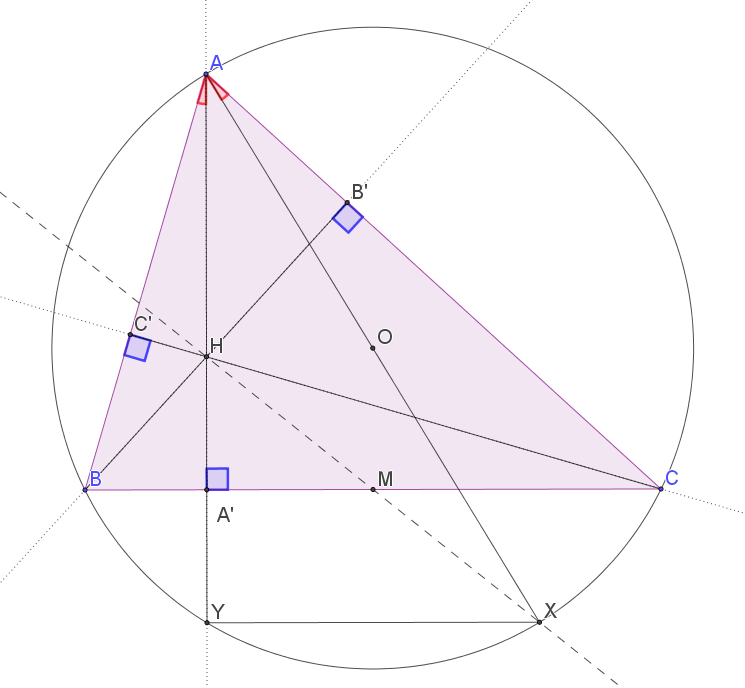
\includegraphics[scale=0.8]{PNAC10.png}
    \end{center}




\section{$I$ y $I_A$}


\subsection{Bisectrices}

Primero vamos a probar que existen, para eso tenemos que ver propiedades de las bisectrices. \\

\begin{definition}
    La bisectriz interior de $\angle BAC$ es la recta  que divide el \'angulo interno en dos iguales.
\end{definition}
\begin{definition}
    La bisectriz exterior de $\angle BAC$ es la recta  que divide el \'angulo exterior en dos iguales.
\end{definition}

Una propiedad a notar es que la bisectriz interior y la exterior son perpendiculares. \\

Estas son como usualmente se piensan estas definiciones, pero en realidad si las tomas juntas son:

\begin{claim}
    Las bisectrices de $\angle BAC$ son el lugar geometrico de los puntos $P$ que equidistan de la recta $AB$ y $AC$. 
\end{claim}

\begin{proof}
    Sean $X,Y$ los pies de altura de $P$ hacia $AB,AC$ podemos notar que $APX, APY$ son congruentes si y solo si $AX=AY$ o $\angle PAX=\angle PAY$. \\
   
    \begin{center}
        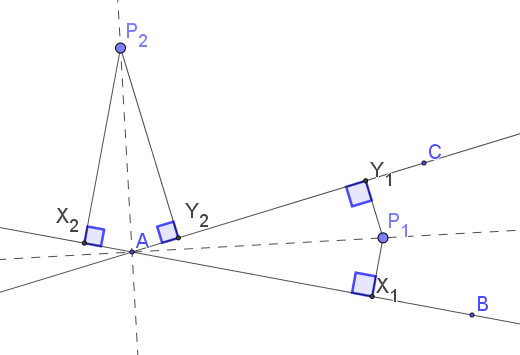
\includegraphics[scale=0.8]{PNAC6.png}
    \end{center}

    Entonces para ver las dos direcciones tenemos que:
    \[\angle PAX=\angle PAY \Rightarrow  APX \cong APY \Rightarrow PX=PY\]
    \'o 
    \[PX=PY \Rightarrow APX \cong APY \Rightarrow \angle PAX=\angle PAY\]
    Probando que un punto equidista a $AB,AC$ si y solo si esta en alguna bisectriz.
\end{proof}

\subsection{$I$ existe}

Ahora veamos que concurren para ver que $I$ existe.

\begin{claim}
    En un triangulo $ABC$ las bisectrices interiores de $\angle BAC, \angle ACB, \angle CBA$ concurren
\end{claim}

\begin{proof}
    Sea $I'$ la interseccion de las bisectrices de $B, C$.
    Sean $D,E,F$ los pies de perpendicular desde $I'$ hacia $BC,CA,AB$.
    
    \begin{center}
        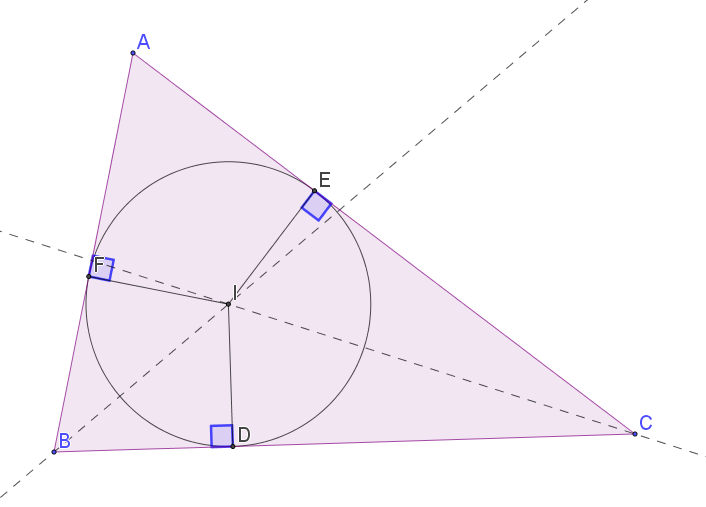
\includegraphics[scale=0.8]{PNAC7.png}
    \end{center}
    
    Entonces como $I'$ esta en la bisectriz de $B$ y $C$ entonces $I'F=I'D$ y $I'D=I'E$ Entonces
    \[I'F=I'D=I'E\]
    y $I'$ esta en la bisectriz interna de $A$, entonces $I'=I$.
\end{proof}

Entonces como $I'F=I'D=I'E=r$, considera el circulo con centro $I$ radio $r$ y pasa por $D,E,F$ adem\'as por los 
\'angulos de $90\dg$ formados con $I$ se tiene que los lados del triangulo $ABC$ son tangentes a ese circulo, el incirculo. \\


Las pruebas para $I_A,I_B,I_C$ son similares.
    \begin{center}
        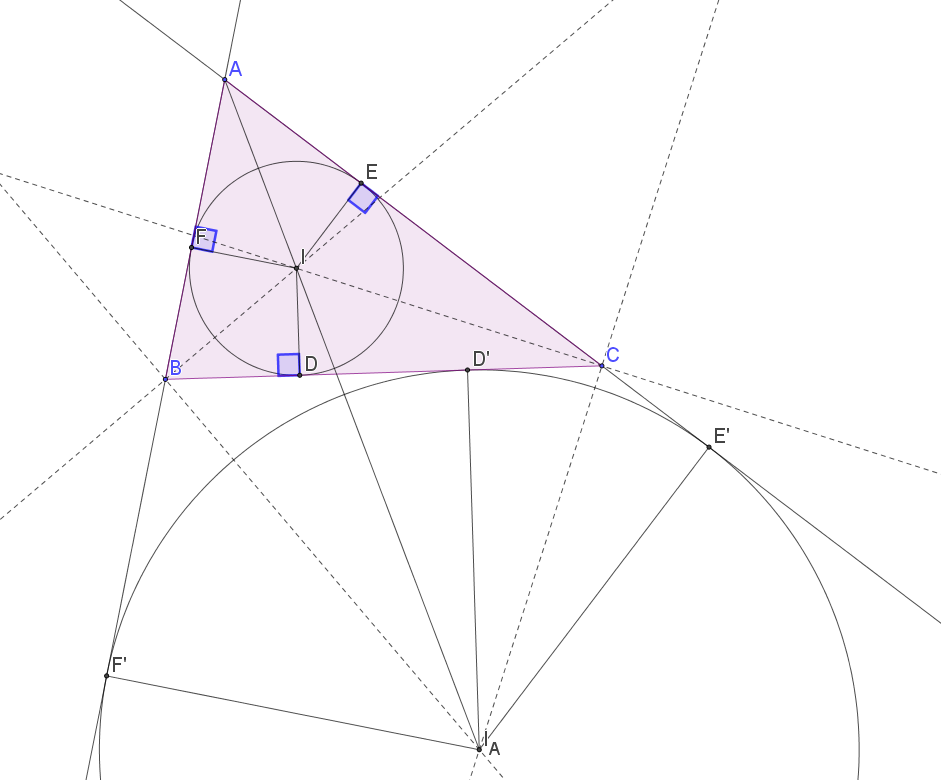
\includegraphics[scale=0.8]{PNAC8.png}
    \end{center}

Algunas propiedades elementarias son:

\begin{itemize}
    \item $AE=AF, BF=BD, CD=CE$
    \item $A, I, I_A$ son colineales
    \item $\angle IBI_A=90\dg$
    \item $AFIE, BDIF, CEID$ son ciclicos.
\end{itemize}

\subsection{Divisi\'on de \'Angulos}

De igual manera que con los centros anteriores podemos dividir los \'angulos, esta vez de la manera \textit{trivial}.

\begin{align*}
    \angle BAI=\angle CAI &= \alpha \\
    \angle ABI= \angle CBI &= \beta \\
    \angle ACI= \angle BCI &= \gamma
\end{align*}



Algo que cumplen es $\alpha+\beta+\gamma=90\dg$

\begin{center}
        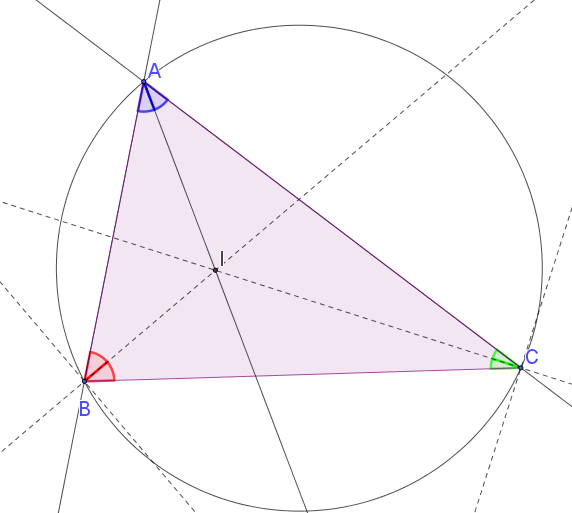
\includegraphics[scale=0.4]{PNAC13.png}
    \end{center}

\subsection{Lema Incentro Excentro}

Para este lema vamos a aprovecharnos de que $\angle IBI_A=90\dg$. \\

Gracias a esta propiedad podemos notar que $IBI_AC$ es ciclico. Adem\'as el 
centro es el punto medio de $II_A$ digamos $J$, por lo tanto $J$ esta en la bisectriz de $A$. \\
Notemos que 

\[\angle AJI= \angle BJI = 2 \angle BCI = \angle BCA\] 
por lo que $ABJC$ es ciclico, entonces el centro 
esta en el circuncirculo, y como esta en la bisectriz es el punto medio del arco $BC$. 

\begin{lemma} [Incentro-Excentro]
    Sea $J$ el punto medio del arco $BC$, entonces $JB=JC=JI=JI_A$, es decir, $J$ es el centro de $BICI_A$.
\end{lemma}

\begin{center}
        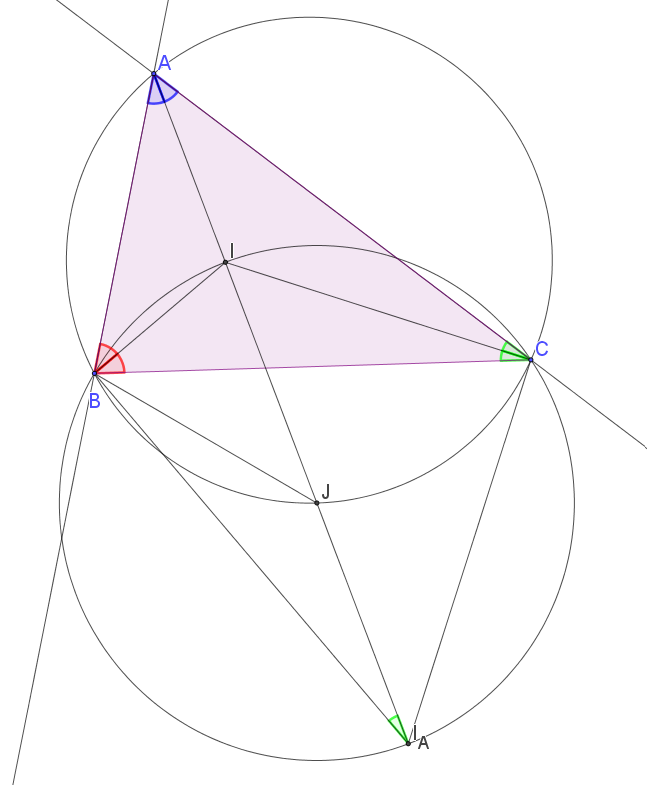
\includegraphics[scale=0.6]{PNAC14.png}
    \end{center}


\newpage

\section{Problemas}
\epigraph{" i'm not ready at all but it's now august 2 and THE SHOW MUST GO ON"
}{Evan Chen}

\begin{problem}[\gad]
Demuestra todas las propiedades que no demostramos en la teoria.
\end{problem}


\problemdiff{1}
\begin{problem}
    Sea $ABC$ un triangulo, sean $D,E,F$ los pies de altura de $A,B,C$ respectivamente. Demuestra que $H$ es el incentro de $DEF$.
\end{problem}

\problemdiff{1}
\begin{problem}
    En un triangulo $ABC$ sean $D,E,F$ los pies de alturas de $A,B,C$, respectivamente. DemFuestra que los triangulos $AEF, BFD, CDE, ABC$ 
    son semejantes entre si.
\end{problem}




\problemdiff{2}
\begin{problem}
Si $I$ es el incentro del triangulo $ABC$ prueba que 
$$\angle BIC =90+\half \angle BAC$$
\end{problem}

\problemdiff{3}
\begin{problem}
Demuestra que en un triangulo $ABC$ el punto medio del arco $BC$ es el circuncentro de $BIC$ pero sin usar nada del excentro (tipo, usando puros \'angulos/propiedades del triangulo solito).
\end{problem}

\problemdiff{2}
\begin{problem}
    Sea $I$ el incentro de un triangulo $ABC$ con $AB<AC$. La linea $AI$ intersecta el circuncirculo de $ABC$ en $D$. El circuncirculo de $CDI$ intersecta $BI$ de nuevo en $K$. Prueba que $BK=CK$.
\end{problem}

\problemdiff{2}
\begin{problem}
    Sea $ABC$ un triangulo acutangulo, sea $K$ la intersecci\'on de la bisectriz interna de $\angle BAC$ y de la mediatriz de $BC$, demuestra que $A,B,C,K$ son conciclicos.
\end{problem}

\problemdiff{2}
\begin{problem}
    Demuestra que $I$ es el ortocentro del triangulo $I_AI_BI_C$.
\end{problem}


\problemdiff{3}
\begin{problem}
    Sea $ABC$ un triangulo. El incirculo de $ABC$ es tangente a $AB, AC$ en $D,E$. Sea $O$ el circuncentro de $BCI$. Demuestra que $\angle ODB=\angle OEC$
\end{problem}

\problemdiff{3.5}
\begin{problem}
    Sea $ABC$ un triangulo acutangulo con circuncentro $O$, sea $K$ un punto tal que $KA$ es tangente al circuncirculo de $ABC$, y $\angle KCB=90\dg$. Un punto $D$ en $BC$
    cumple que $KD \parallel AB$, demuestra que $A,O,D$ son colineales.
\end{problem}

\problemdiff{3.5}
\begin{problem} [9 puntos]
    Demuestra que en un triangulo $ABC$, los puntos medios de $AH,BH,CH,AB,BC,CA$ y los pies de altura $A',B',C'$ son todos conciclicos. (Con angulos)
\end{problem}


\problemdiff{4}
\begin{problem} [OTIS]
Sea $ABC$ un triangulo con circuncentro $O$ y ortocentro $H$. Prueba que $AO=AH$ si y solo si $\angle BAC=60$
\end{problem}




\problemdiff{5}
\begin{problem} [\gad]
    Sea $ABC$ un triangulo acutangulo, sea $D$ el pie de altura desde $C$. La bisectriz de $\angle ABC$ intersecta $CD$ en $E$ e intersecta al circuncirculo $\omega$ de $ADE$ en $F$. Si $\angle ADF=45$ muestra que $CF$ es tangente a $\omega$.
\end{problem}

\problemdiff{5}
\begin{problem}[AoPS] %isaac
    Sea $ABC$ un triangulo acutangulo con circuncirculo $\omega$ y sea $O$ el centro de $\omega$. $M$ es el punto medio de $BC$, $H$ el ortocentro, $BE$ la altura, $\ell$ es una recta que pasa por $E$
    y es perpendicular a $ME$. El rayo $MH$ intersecta a $\omega$ en $Q$, $BE$ intersecta $\omega$ en $B$ y $N$. $QN$ intersecta $\ell$ en $P$. Prueba que $C,O,P$ son colineales.
\end{problem}

\end{document}